\documentclass{article}
\usepackage[utf8]{inputenc}
\usepackage{hyperref}
\usepackage{url}
\usepackage{mathtools}
\usepackage{amsmath}
\usepackage{graphicx}
\usepackage{wrapfig}
\usepackage{algorithm}
\usepackage{algpseudocode}
\usepackage{subcaption}
\usepackage[svgnames]{xcolor}
\usepackage{listings}
\usepackage[left=2.5cm, right=2.5cm, top=1.5cm, bottom=2cm]{geometry}
\setcounter{section}{-1}


\title{
\textbf{Algorithmics for Data Mining: Deliverable 3\\} \Large{
    Democrat Vs. Republican Tweets}}
\author{Oriol Borrell\\
\textit{\small FIB - UPC Student} \\
\textit{\small Barcelona, Spain} \\
\textit{\texttt{\href{mailto:oriol.borrell.roig@est.fib.upc.edu}
{\small oriol.borrell.roig@est.fib.upc.edu}}}}
\date{\today}

\begin{document}
\maketitle

\section{Abstract}

\textit{
We will analyze what do politicians of the Republican and Democrat Parties (in USA) tweet about. We will first see if we can extract any conclusion about particularities of each party tweet. Afterwords we will train a model that will predict, given a tweet, if it belongs to the Republican or to the Democrat party.
The Code for this project can be founded here \footnote{Github repository of the project: \url{https://github.com/oriolborrellroig/ADM-Deliveries/tree/master/ThirdDelivery}}. The data was extracted from here \footnote{Data used in the project: \url{https://github.com/suneman/socialgraphs2019/tree/master/files/data_twitter}}
}

\section{Context}
\label{Context}
The tweets obtained are all tweets from 2019 created by different USA politician's. We have to take into account that Donald Trump (from the Republican party) is the president of USA since January 20, 2017. The 2019 in USA was a Off-year election.

Republicans and Democrats are the two main and historically the largest political parties in the US. After every election, they hold the majority seats in the House of Representatives and the Senate as well as the highest number of Governors.

\section{What do Democrat and Republican members tweet about?}
\label{sec:Wordcloud}

Before analyze the tweets we applied the following preprocessing steps:
\begin{itemize}
    \item Remove the newline characters
    \item Remove commonly used ampersand
    \item Remove ' from contractions such as I'm and don't
    \item Lowercase the string
    \item Remove https-links from the string
    \item Tokenize the strings
\end{itemize}

Once we had the tokens, we computed the frequencies of each token in each party. We created the wordcloud shown in Figure \ref{fig:WordCloud100}.

\begin{figure}[H]
    \centering
    \begin{subfigure}{.8\textwidth}
        \centering
        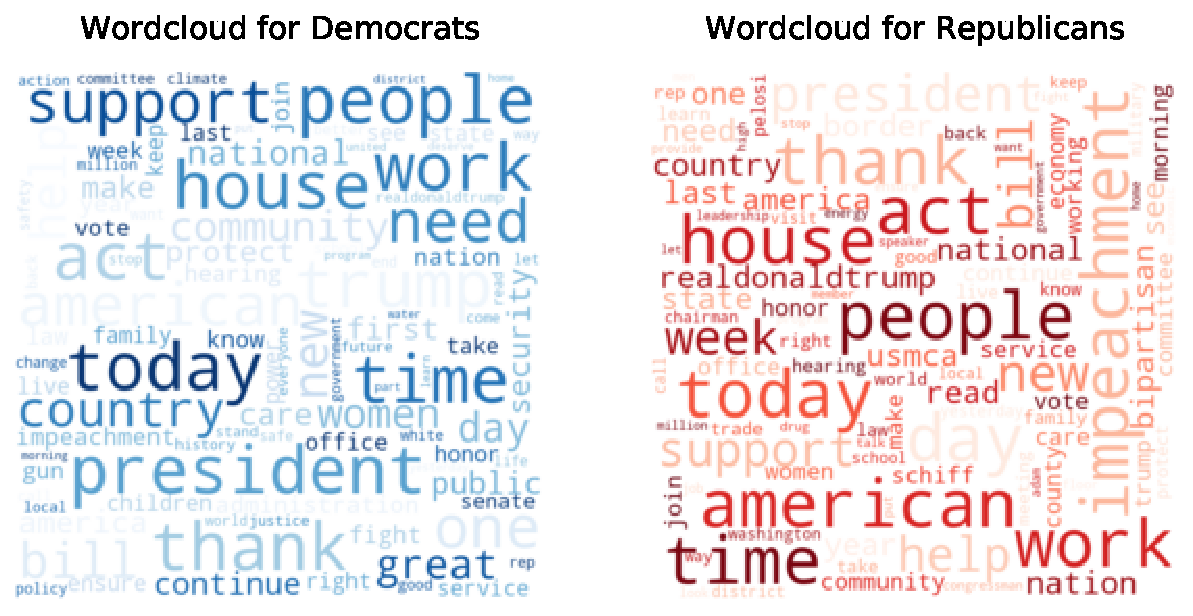
\includegraphics[width=1\textwidth]{./img/WordCloud100.pdf}
    \end{subfigure}
    \caption{Wordcloud of the top used tokens of each party}
    \label{fig:WordCloud100}
\end{figure}

Analyzing the results, we observe that the most used words of each party are fairly common words in the field of politics. We cannot extract any particularity neither from the Democrats nor Republicans.

Doing a bit of research I founded a common concept in \textit{Information Retival} called \textit{Term Frequency–Inverse Document Frequency, TFIDF\footnote{TFIDF's Wikipedia page: \url{https://en.wikipedia.org/wiki/Tf-idf}}}. TFIDF is a way to compute the importance a word is in a document. As shown in Equation \ref{eq:TFIDF} is computed using two statics, the \textit{Term Frequency(tf)}, and the \textit{Inverse document frequency(idf)}:

\begin{equation} \label{eq:TFIDF}
    \begin{split}
        & tf(t,d) = 0.5 + 0.5\times \frac{f_{t,d}}{max\{f_{t^{'},d}: t^{'} \in d\}} \\
        & idf(t,D) = log \frac{N}{|d\in D:t\in d|} \\ \\
        & tfidf(t,d,D)  = tf(t,d)\times idf(t,D) 
    \end{split}
\end{equation}

Where $f_{t,d}$ is the frequency of the token \textit{t} in the document \textit{d}, and $N$ is the total number of documents in the collection $D$.

We computed this static for each word and created another time the wordcloud of each party. The results are shown in Figure \ref{fig:WordCloudTFIDF}

\begin{figure}[H]
    \centering
    \begin{subfigure}{.8\textwidth}
        \centering
        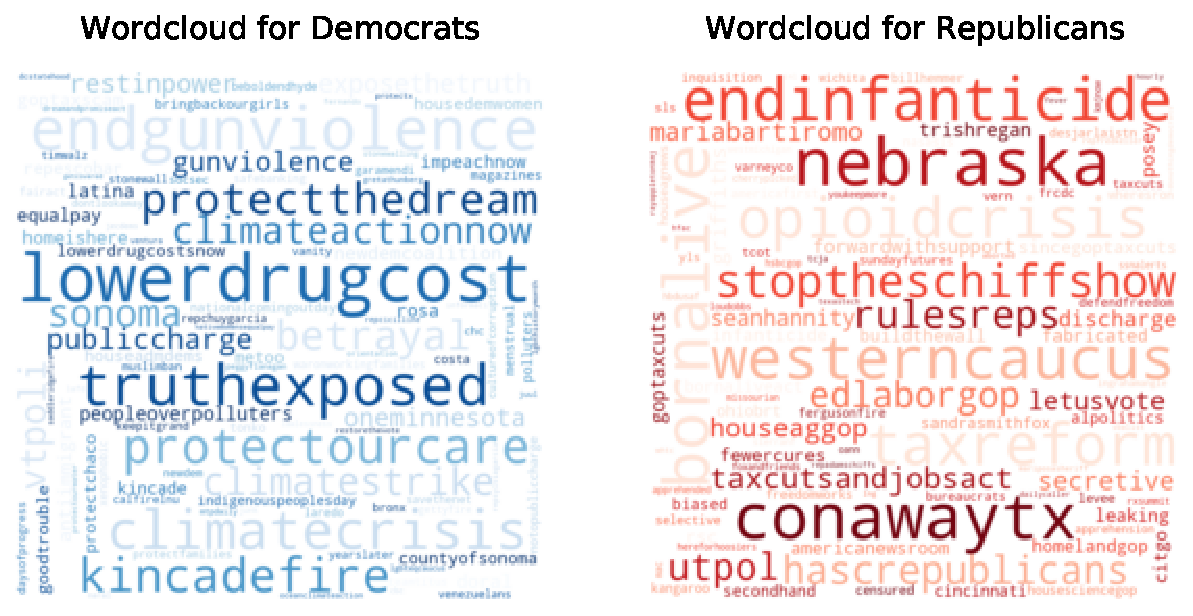
\includegraphics[width=1\textwidth]{./img/WordCloudTFIDF.pdf}
    \end{subfigure}
    \caption{Wordcloud using TFIDF}
    \label{fig:WordCloudTFIDF}
\end{figure}


The obtained wordclouds are very interesting. We see that the Democrats apparently have a larger focus on \textit{climate} and \textit{health care} where the Republicans focus on \textit{anti-abortion} and \textit{tax-cuts}. These topics are all more interesting and polarizing than the previous results, where we saw that both parties often referred to different political personalities, committees and other political jargon. We see a clear indicator, that the phrases for both parties are political slogans, such as \textit{endgunviolence} and \textit{bornalive}. Twitter, therefore, gives us a valuable insight into the key-issues and focal points of each party.

\section{Predicting the party of a tweet}
\label{CNN}

In order to predict the party of a tweet we trained a Convolutional Newral Network (CNN). We applied the same preprocessing steps mentioned before in order to obtain the tokens. Once obtained the token, I substituted each token with their position in a top used words ranking, or 0 if it's not a frequently used word. With this substitution I obtained continues numerical data that I could send-it to te model.

About the model, in other deliveries I briefly explained the behavior of a CNN and the different types of layers. I will assume this knowledge is already explained. The following table shows the CNN I designed:

\begin{table}[ht]
    \centering
    \begin{tabular}{|l|ccc|}
        \hline
        \textbf{Layer(type)} & \textbf{Units} & \textbf{Filter} & \textbf{Stride} \\
        \hline
        Embedding & - & - & - \\ \hline
        Conv1D & 32 & 3 & 1\\ \hline
        MaxPooling1D & - & 3 & 2\\ \hline
        LSTM & - & - & -\\ \hline
        Dense & 5 & - & -\\ \hline

    \end{tabular}
    \caption{CNN Layers}
    \label{tab:CNN_Layers}
\end{table}

Once trained the model we tested with the 20\% of data that we reserved for this purpose. We obtained a accuracy of 0.74. 

\section{Conclusions}
Personally, I think that spending more time trying to build the model with different layers or parametrization, or founding a better wey to convert the tokens into numeric data, could lead us to achieve a better accuracy. Is the first time I work with text data, and the project helped me to learn steps that are important to apply, and useful statics when dealing with this type of data.

However, the results obtained in Section \ref{sec:Wordcloud}, in my opinion are very powerful, and reveal the main priorities and way of think of each party in some political topics. 

\end{document}
